\section{RESULTS}
% Edit below
Tussentitels per topic/techniek (4.1, 4.1.1, \dots).
Beschrijf de resultaten (interpreteer ze nog niet), wat zie je (objectief)?
Zorg dat figuren een caption hebben (incl. alle afkortingen) onder de figuur en dat je zeker in de tekst refereert naar desbetreffende figuur. 
Tabellen krijgen een caption bovenaan (zelfde principe).

Willen jullie resultaten tonen zoals figuren dan dienen jullie de \textit{figure} environment gebruiken.

\begin{figure}[!htpb]
    \centering
    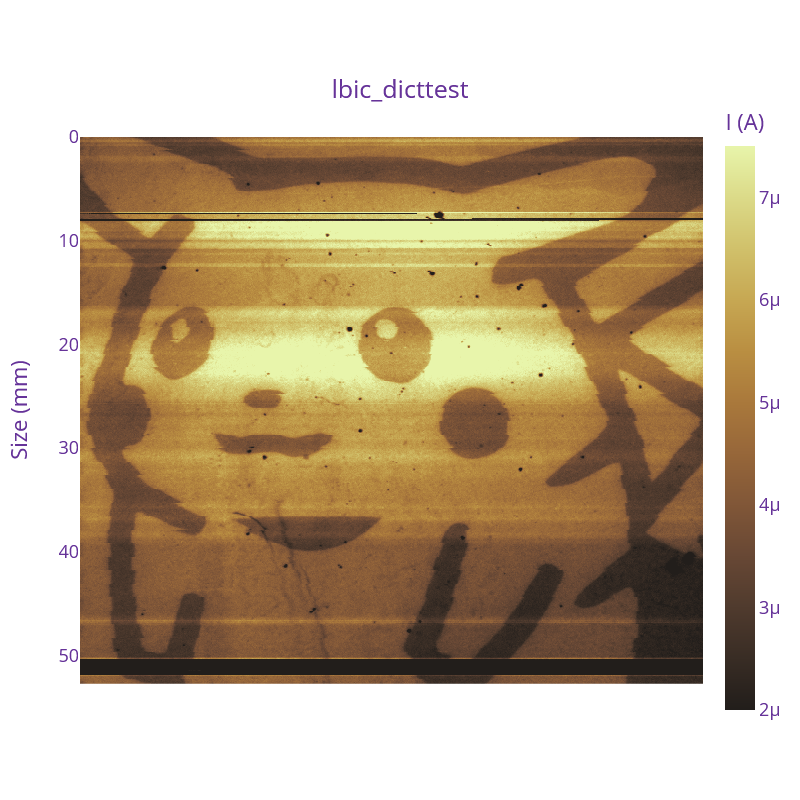
\includegraphics[width=\linewidth]{Figures/newplot(4).png}
    \caption{Dit is het onderschrift van deze figuur}
    \label{fig:pikachu}
\end{figure}

Je kan naar een figuur refereren met \lstinline!\cref{fig:pikachu}! door een label te plaatsen in je figure environment: \lstinline!\label{fig:pikachu}!.
Ook andere objecten kunnen een label hebben, zo kan ik bijvoorbeeld verwijzen naar \cref{eq:ne}.
\Cref{fig:p1,fig:p2} toont hoe eventueel gebruik gemaakt kan worden van \textit{minipage} voor twee zij-aan-zij figuren.

\begin{figure*}
    \centering
    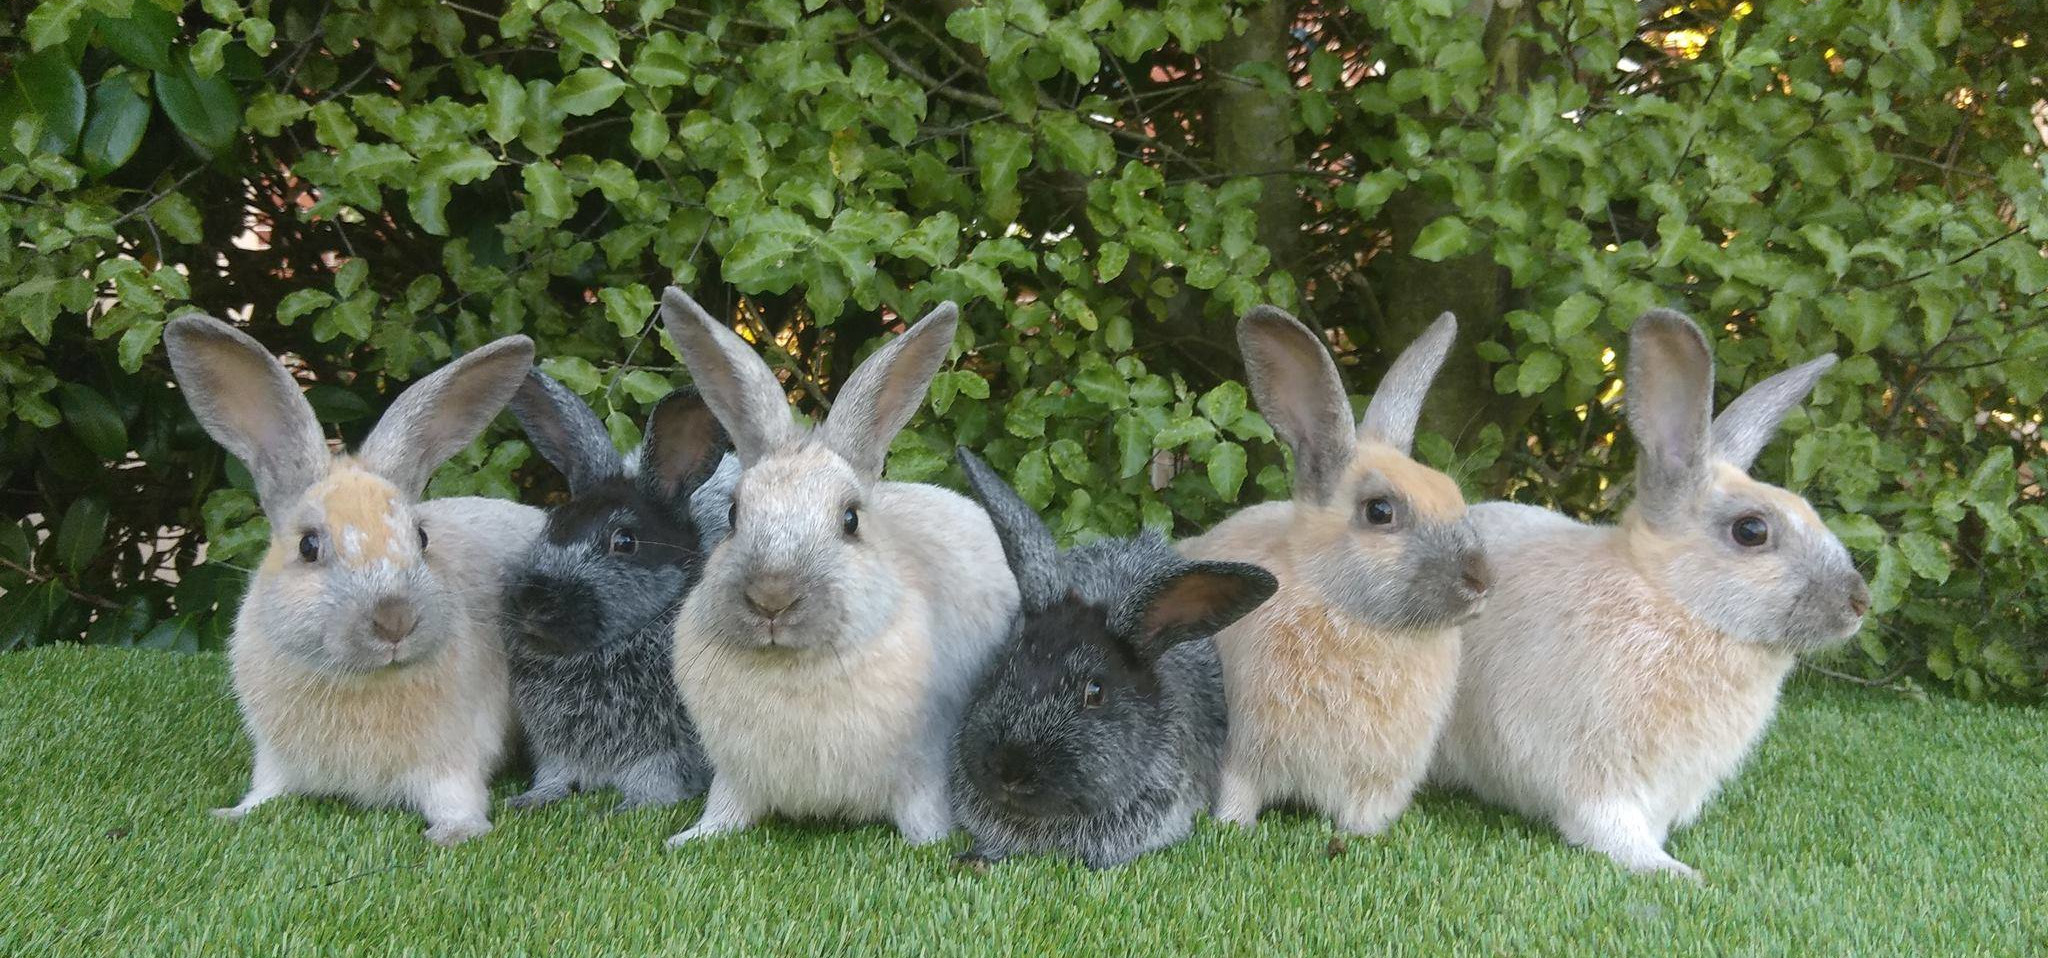
\includegraphics[width=\textwidth]{Figures/Enderby_Island_Rabbit_Lineup.jpg}
    \caption{Dit is een veel te grote figuur. Konijnen zijn belangrijk en moeten de hele pagina innemen.}
    \label{fig:konijnen}
\end{figure*}
Grote figuren kunnen verspreid worden over de twee kolommen door gebruik van \lstinline!\begin{figure*}! zoals in \cref{fig:konijnen}. 

\begin{figure*}
    \centering
    \begin{minipage}{0.45\textwidth}
        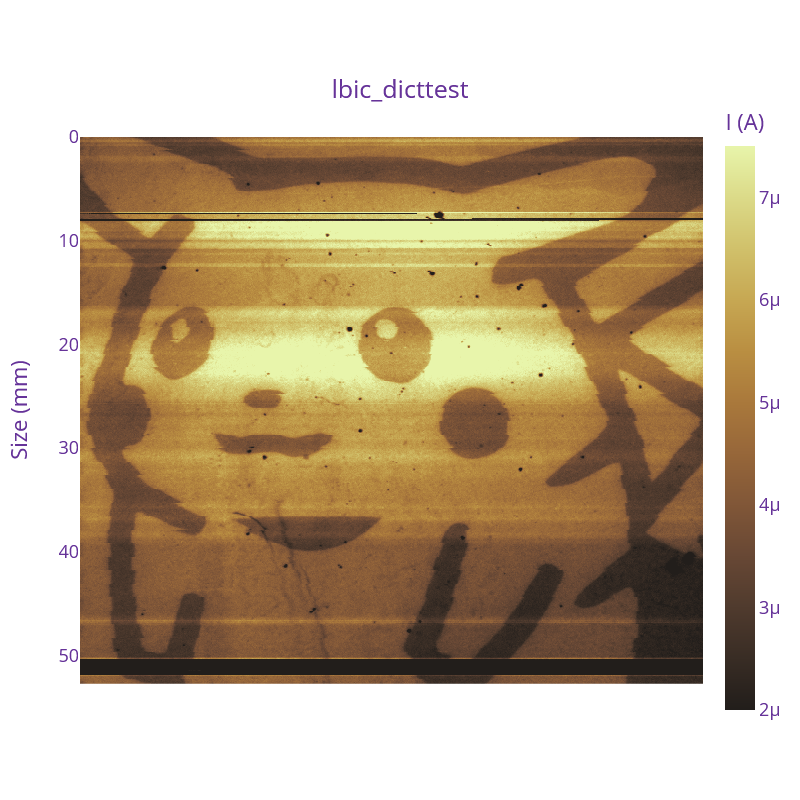
\includegraphics[width=\linewidth]{Figures/newplot(4).png}
        \caption{Dit is het onderschrift van deze figuur}
        \label{fig:p1}
    \end{minipage}
    \hspace{0.05\textwidth}
    \begin{minipage}{0.45\textwidth}
        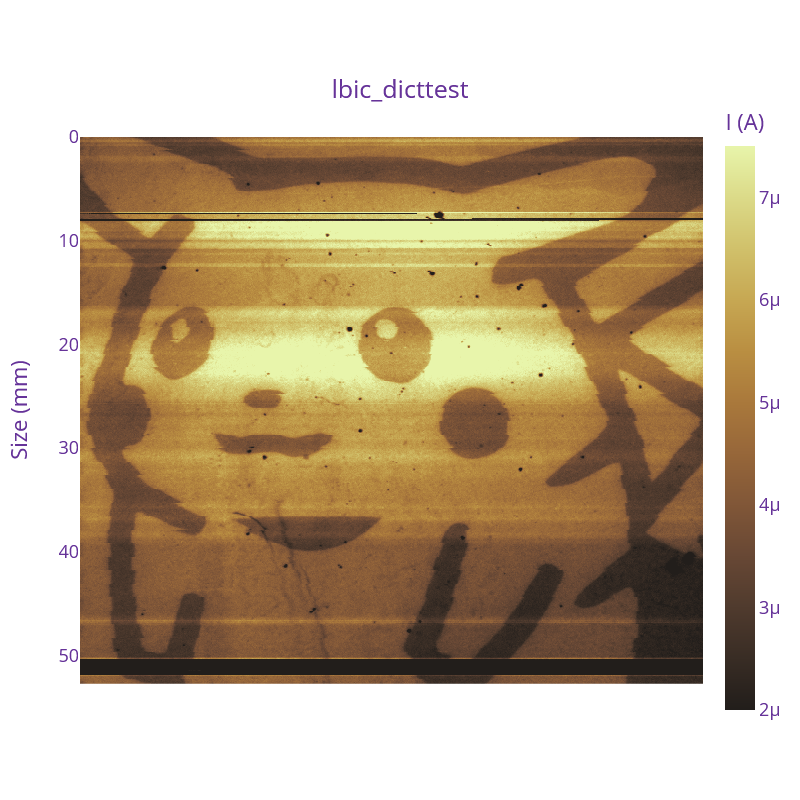
\includegraphics[width=\linewidth]{Figures/newplot(4).png}
        \caption{Dit is het onderschrift van deze figuur}
        \label{fig:p2}
    \end{minipage}
\end{figure*}

Tabellen moeten in de \textit{table} environment geplaatst worden.
Ook hier is de 'H' parameter cruciaal.
Gebruik \url{https://www.tablesgenerator.com/} voor hulp bij de opmaak van tabellen.

\begin{table}[!htpb]
\centering
    \label{tab:example_table}
    \caption{Example table with no meaning}
    \begin{tabular}{||c c c c||} 
    \hline
    Col1 & Col2 & Col2 & Col3 \\ [0.5ex] 
    \hline\hline
    1 & 6 & 87837 & 787 \\ 
    2 & 7 & 78 & 5415 \\
    3 & 545 & 778 & 7507 \\
    4 & 545 & 18744 & 7560 \\
    5 & 88 & 788 & 6344 \\ [1ex] 
    \hline
    \end{tabular}
\end{table}